\documentclass[11pt]{book}

\usepackage[width=7.0in, height=9.0in, top=1.0in, papersize={8.5in,11in}]{geometry}
\usepackage[pdftex]{graphicx}
%\usepackage{datetime}
\usepackage{anyfontsize}
\usepackage{t1enc}
\usepackage{verbatim}
\usepackage{algorithm}
\usepackage{algorithmic}
\usepackage{framed}
\usepackage{pdfpages}
\usepackage{listings}
\lstset{language=C}

\lstset{language=python,frame=ltrb,framesep=5pt,basicstyle=\normalsize,
 keywordstyle=\ttfamily\color{DarkRed},
%morecomment=[n][\textbf]{In\ [}{]\:},
%morecomment=[n][\textbf]{Out\ [}{]\:},
morecomment=[s][\color{blue}]{In\ [}{]\:},
morecomment=[s][\color{red}]{Out[}{]\:},
identifierstyle=\ttfamily\color{DarkBlue}\bfseries,
commentstyle=\color{DarkGreen},
stringstyle=\ttfamily,
showstringspaces=false,tabsize = 3}


\lstdefinelanguage{shell} {
commentstyle = \color{black},
keywordstyle = \color{black},
stringstyle = \color{black},
identifierstyle = \color{black},
morecomment=[s][\color{blue}]{In\ [}{]\:},
morecomment=[s][\color{red}]{Out[}{]\:},
 }

\pagestyle{empty}

\usepackage{helvet}
\renewcommand{\familydefault}{\sfdefault}

\begin{document}

\fontsize{16}{16}\selectfont Sprint Report \#2


\section{Team Members:}
Marcus Berger
\\Dicheng Wu\\
\textbf{Sponsor:}
\\Jeff McGough
\\

\section{Prototype Progress}
The progress is being made on the simpler functions of the projects including search, updates, and role sheets. As of now the prototype is in a state of some working functionality on the admin and teacher side. The pages are not yet tied together but the complete functions function independently. Several GUI pages are complete or in a working state to compliment these functions. The back end database has been slightly updated to adjust to the needs of the project. Lastly the prototype has reached a state where testing can be conducted on parts of the project, more information is given later in this document.

\section{Project deliverables of Sprint 3:}

\begin{enumerate}
\item Student search page 
\item Employee search page
\item Add a class to the database
\item Update teacher and student information pages
\item Modify clothing requirements for a class
\item Generate a class role sheet
\item Assign teacher to a class
\item Ability to add and subtract students from a class  
\end{enumerate}


\subsection{Sprint 3 Backlog:}

\begin{enumerate}
\item Queries in database to retrieve student and employee information
\item Query and insert information needed to create and new class and produce a results page.
\item Query database to produce class role sheet
\item Create clothing requirement update function, and add clothing function for teachers and admin
\item Create update query to assign teachers to a class
\item Create ability for employee to look up and modify student registration info
\item Add and subtract students from a class
\item Sprint 3 Review
\item Create Client presentation
\item Documentation for semester
\end{enumerate}

\section{Search Pages}
The first page tackled this sprint was the search page. The page takes user input and searches based on name using a fuzzy search. Also included in both searches is an advanced search option that allows the user to check boxes corresponding to the fields in the database, which allows the user to search in more versatile ways. Lastly the user can click on a student to pull up all of their information and modify it as needed.


\begin{figure}
\caption{Search Pages}
\centering
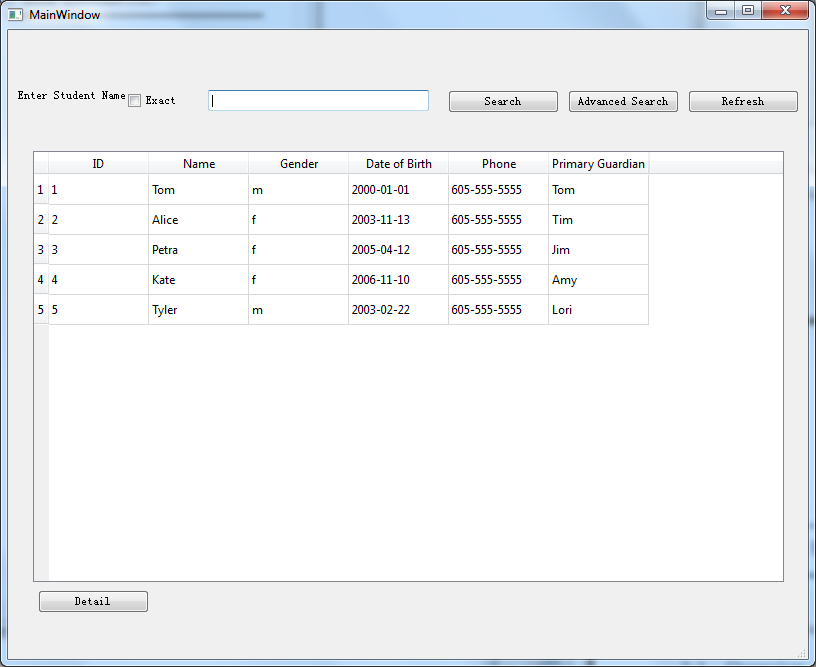
\includegraphics[width=0.5\textwidth]{search}
\end{figure}

\section{Add A Class}
Clicking on the "Add a Class" button on the admin landing page will open a dialog. From this dialog box the user can type in information to a add a class. These fields include class name, cost, start and end times, day, clothing requirements, class description, start and end dates, and the age range for the class.  At the time of class creation only name, is a required field. When the submit button is clicked a message box will pop up to confirm the database submission before submitting to the database  

\section{Role Sheet}

\section{Update Pages}
These pages are fairly simple to explain sometimes the user will need to add or alter a record of some kind these pages need to be able to do that in a simple and concise way. The update pages worked on in this sprint include student information from the employee side, updating teacher information and updates to clothing requirements for a class. Most of these page will just produce a form where information can be displayed and updated.

\section{Assign Teacher to a Class}
This page allows an admin to select a class, clicking on a class pulls up a list of available teachers to select to teach the class. Clicking on a teacher will pull up a message box to confirm the selections before submitting to the database. The available teachers are selected based on the start time of the selected class and the end time of the classes already being taught by each teacher. If the class times overlap then that teacher will not show up in the available teachers list.

\section{Sprint 3 Issues}
Some issues that were encountered during this sprint were:

\begin{enumerate}
\item Time - While not as much of a problem as it was in sprint two the group still found itself running low on time. The lead gained during Christmas break should reduce the issue in phase 2.
\item Inexperience with pyqt - While still a small issue the experience of the team is growing and while some issues still exist such as needing to look up information at times, the issues are lessened from the last sprint.
\item Team communication - The team found some issues in communicating with one another because of other projects and assignments. Which in some cases slowed sprint progress. Mitigation for this issue will be to more strongly impose a schedule in phase 2.
\end{enumerate}

\section{Client Interactions}

Client interactions came in the form of weekly meeting every Wednesday at 2:00 p.m. Topics included:

\begin{enumerate}
\item Progress reports on where we are in the project
\item Asking questions to refine functionality and understand academy needs
\item Discuss the future of the project and idea on how to execute them
\end{enumerate}


\section{Group Meeting}

The group has a standard meeting time of TTH 10:00 - 12:00 and once during the weekend usually from 1:00-5:00 

Meeting can continue pass these times if needed, and other times during the weekend. However extra weekend times fluctuate and do not remain constant from week to week. 

\section{Work Distribution}

Marcus:
\begin{enumerate}
\item Add a class
\item Assign teacher to class
\item Update teacher page
\item Update clothing
\item documentation
\item trello management\\
\end{enumerate}

Dicheng:
\begin{enumerate}
\item Search Pages
\item Role sheet
\item Modify student information
\item Add and Subtract students from a class\\
\end{enumerate}


Together:
\begin{enumerate}
\item Updated database construction
\item GUI page breakdown based on user stories and product backlog
\item Coded some functionality
\end{enumerate}

\end{document}